\chapter{Application Programming Interface (API)} \label{sec:API}

Section \ref{sec:classesRelations} gives the details of the Mesquite paradigm. That section does not
delve into details and should be read before writing a driver code in order to master the basic
concepts. 

Section \ref{sec:detailedAPI} delves into the details of the various concrete classes available in
Mesquite. The syntaxic details of the API are given in the user doxygen doc available by running
'doxygen Mesquite-user.dox' in the directory mesquite/doc/user/doxygen. 

\section{Relations between the Mesquite API Classes} \label{sec:classesRelations}

The Mesquite architecture, shown in Figure \ref{fig:uml}, closely
follows the abstractions of the optimization problem defined in \ref{sec:concepts}.
In particular, the core abstract classes needed to
define a mesh quality improvement algorithm are {\tt QualityMetric},
{\tt ObjectiveFunction} (which takes a {\tt QualityMetric} as
input), and {\tt QualityImprover} (which takes an {\tt ObjectiveFunction}
as input).

In addition, a number of other classes have been created to support
the needs of mesh quality improvement algorithms:
\begin{itemize}
\item {\tt QualityAssessor}: to provide an evaluation of mesh
quality using standard statistical procedures,
\item {\tt TerminationCriterion}: to customize the stopping criteria
used with a mesh quality improvement algorithm,
\item {\tt InstructionQueue}: to compose quality improvers and
quality assessors together to form efficient mesh quality improvement
and evaluation methods, and
%\item {\tt MeshSet} and {\tt PatchData}: to provide the mechanisms
%for managing the application mesh and geometry information and the
%mesh sub-domains used in optimization procedures.
\end{itemize}

\subsection{UML Diagram}

\begin{figure*}[htbp]
\begin{center}
    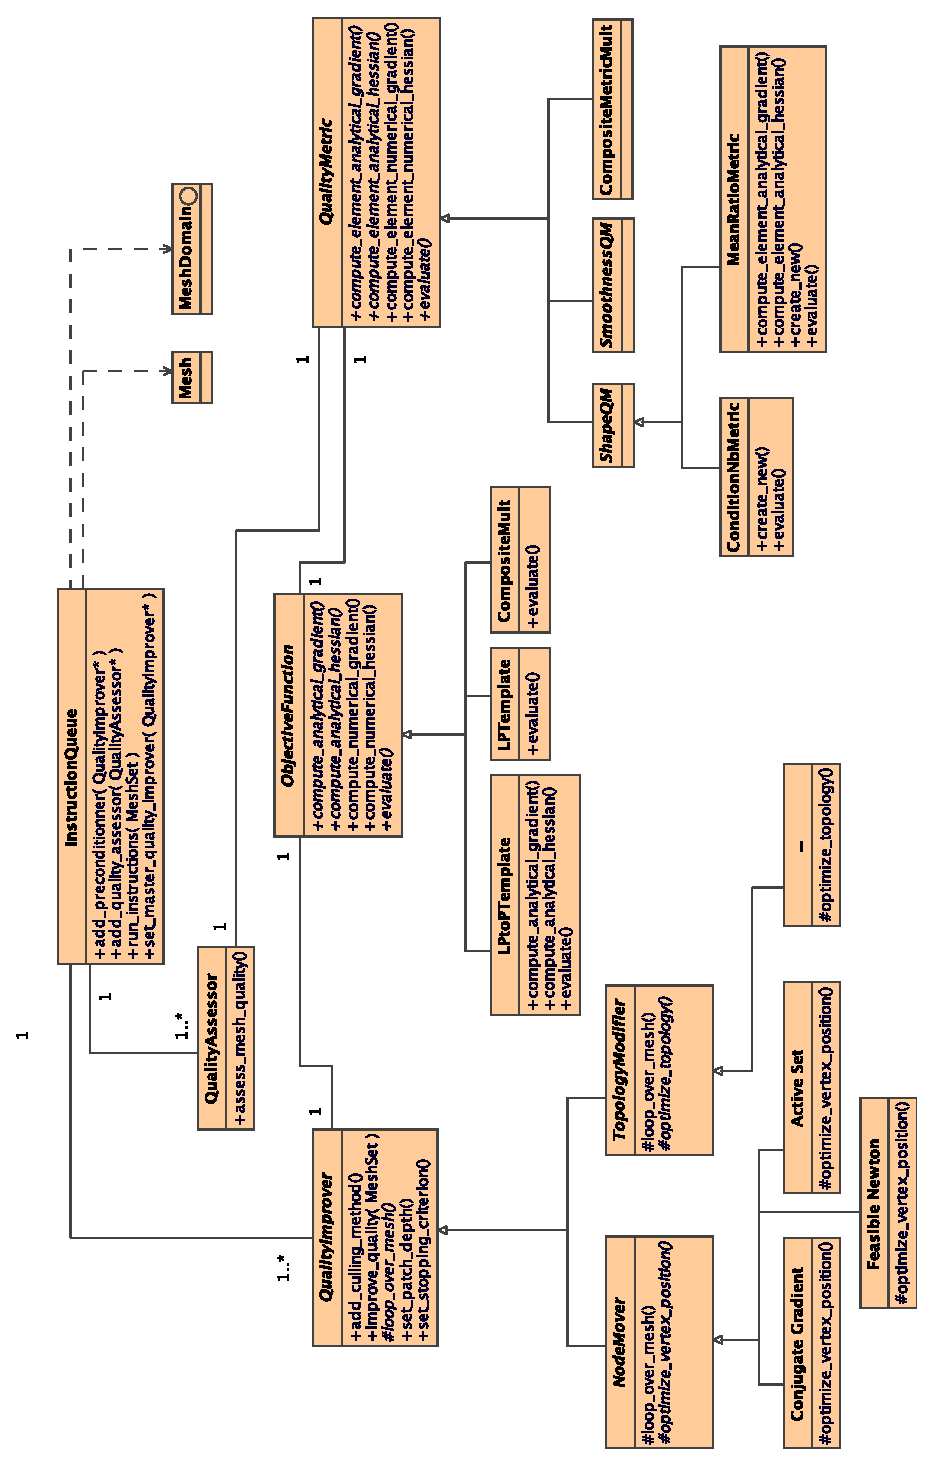
\includegraphics{MesquiteUI.eps}
    \caption{Mesquite user interface UML class diagram.  Abstract
             classes and virtual functions are in italic. Vertical
             links with a triangle indicate inheritance. Plain links
             indicate association. Protected functions are prefixed
             with '\#', public ones with '+' .}
    \label{fig:uml}
\end{center}
\end{figure*}

The UML diagram in figure \ref{fig:uml} presents the layout of the Mesquite classes. It should be
looked over once now, and then examined in more details when each class is described in the
following subsections.


\subsection{The Quality Metric -- Objective Function -- Quality Improver Trio} 
\label{sec:trio}

In the following sections, we will use the notations introduced in section \ref{sec:concepts}. 

Improving a mesh with Mesquite consists mainly in selecting three components: the quality metric,
the objective function template, ans the quality improver (i.e. the optimization algorithm). 

The quality metric $q$ describes what the user considers to be a good mesh element as a function of
its vertices coodinates, and possibly other factors such as its proximity to a boundary or an
equivalent element in a reference mesh. The various quality metrics available are described in
section \ref{sec:QualityMetric} and how to implement a new quality metric is described in section
\ref{sec:QualityMetricImpl}.

Now that the element quality has been defined, a template objective function $f$ (section
\ref{sec:ObjectiveFunction}) must be chosen to formulate the mesh we aim for. Do we want to improve
the worst elements, or to make the mesh as good as possible in average ? The combination of the
quality metric and the template objective function give us the mesh quality objective function $F=f
\circ q$.

This mesh quality objective function can now be minimized chosing an optimization algorithm
(\texttt{QualityImprover}), 
a crucial component of the Mesquite framework.  The two main types of improvement schemes
designed into Mesquite are {\tt VertexMover} (see section \ref{sec:VertexMover}) and {\tt
TopologyModifier} (\ref{sec:TopologyModifier}) for vertex relocation or topology modification,
respectively.  These methods take as input a mesh quality objective function ($F=f \circ q$).
The concrete \texttt{QualityImprover} always acts on an
\texttt{ObjectiveFunction} pointer to retrieve the function value and
gradient $\nabla F$, and sometimes the Hessian ${\cal H} F$, for a certain mesh and concrete \texttt{ObjectiveFunction} /
\texttt{QualityMetric} combination.  Dynamic polymorphism ensures at
runtime that the correct evaluations are performed.


\subsection{Termination Criterion}
\label{termination_section}

Mesquite's \texttt{TerminationCriterion} class contains functionality
to customize the termination of the mesh quality improvement process. 
Mesquite wrappers (section \ref{sec:wrappers}) already have an embedded default termination
criterion. The termination criterion provides an automatic mechanism to stop an optimization
procedure. --- familiar examples  comes to mind such as the objective function gradient norm close
to zero in a non-linear programming problem. Many other criterions are available in Mesquite (see
section \ref{sec:TerminationCriterion}). When using the detailed API, termination criterions have to
be set in order for the quality improver to terminate. 
 

\subsection{Quality Assessors}

Mesquite's \texttt{QualityAssessor} class encapsulates functionality to
evaluate quality metric values for a given mesh, to accumulate
statistical information about those values, and to report that data to
the user.  In particular, a \texttt{QualityAssessor} object takes a
{\tt QualityMetric} class as input to evaluate a given mesh and then
reports information like the maximum, average, and standard deviation
of those values.

% \subsection{Culling Capabilities} \label{sec:culling}
% Mesquite includes methods called {\it culling} schemes
% which are intended to decrease the time it takes for the
% quality improvers to reach an adequate mesh.  These schemes
% the mporarily fix the positions of certain vertices which
%satisfy a given culling criteria.  These fixed vertices
%are said to be {\it culled} from the optimization procedure.
%This reduces the number of variables in the optimization
%problem, and therefore this modified problem can often
%be solved in significantly less time than the original problem.  
% LAF - there are no details here - it's not worth including as is

%\subsection{Mesh Data Classes} \label{sec:MeshData}
%There are two mesh data classes in Mesquite, \texttt{MeshSet} and
%\texttt{PatchData}, which have been designed to meet two different
%needs.  The {\tt MeshSet} class is a container that holds pointers, or
%handles, to the meshes provided by the application.  It also provides
%the mechanisms necessary to obtain the mesh information from the
%application through a well-defined, flexible API (see Section
%\ref{sec:meshset}).  To minimize the memory footprint of the Mesquite
%library, only detailed information for the optimization procedure
%subdomains is stored at any given time in the {\tt PatchData} class.
%One or more {\tt PatchData} objects can be originated from the {\tt
%MeshSet} object, and {\tt PatchData} obtains detailed mesh
%information, such as vertex coordinates and element connectivity,
%through the MeshSet accessor functionality.  The \texttt{PatchData}
%class makes Mesquite scalable in that prohibitive memory costs
%associated with making a copy of a large application mesh can be
%avoided by dividing the mesh into patches on which to perform the
%optimization sequentially.
%\subsubsection{MeshSet Interactions with Application Meshes}
%\label{sec:meshset}
%\subsubsection{PatchData Interactions with QualityImprovers}
%Quality improvers are written to relocate nodes or modify topology
%within a \texttt{PatchData}, without any need to know whether the
%\texttt{PatchData} corresponds to the whole mesh or a subset of
%it. The \texttt{PatchData} information is generated by the
%\texttt{MeshSet} class with the \texttt{get\_next\_patch} function ---
%the equivalent of an iterator over a series of patches covering the
%mesh.  The user can set Mesquite to use different types of
%\texttt{PatchData}, ranging from a patch of elements containing one
%particular vertex to a patch of vertices connected to a central vertex
%through edges or a unique patch that covers the whole MeshSet
%(recall that this could be the union of several meshes added by the
%application to \texttt{MeshSet}).

%\texttt{PatchData} and its associated classes
%(e.g. \texttt{PatchDataVerticesMemento}) provides much functionality
%to the optimization algorithms.  Memento patterns can remember the
%state of a \texttt{PatchData} geometry or topology at a given
%iteration and restore the \texttt{PatchData} to that state
%later. Simple functions can move the \texttt{PatchData} $n$ vertices
%in a direction $d \in \Bbb{R}^{3n}$ while constraining the boundary
%vertices to their geometrical surface.

\subsection{The Instruction Queue} \label{sec:IQ}

The \texttt{InstructionQueue} class allows a sequence of operations
such as quality assessment and quality improvement to be performed on
a \texttt{MeshSet} object. The \texttt{InstructionQueue} 
provides a convenient framework to shield the user
from the algorithm syntax and to ensure a consistent use of the
Mesquite capabilities.  One or more quality improvers can be
associated with an {\tt InstructionQueue}, but one must be designated
as the {\it master} quality improver that determines the ultimate 
improvement goal.  All progress made by Mesquite will be
measured against the quality metrics set in the master quality
improver.  To improve the effectiveness and efficiency of the mesh
quality improvement process, several quality improvers can be used as
'pre-conditioners' for the master quality improver.  For example, a
user may precede an optimization-based master quality improver with a
mesh untangler and/or Laplacian smoothing.

Some predefined \texttt{InstructionQueue} objects, called \emph
{wrappers}, are available for high-level or novice users. Those
typically consist of a quality assessor, followed by a mesh
pre-conditioner such as an untangler, followed by a master quality
improver, and finally another quality assessor.  Once an
InstructionQueue has been defined, a single call to \texttt{run\_instructions} 
will perform all the contained operations.  We note
that once an \texttt{InstructionQueue} has been defined, it can be used
for several \texttt{MeshSet} objects.


\section{Simplified Application Programming Interface}
\label{sec:wrappers}
To improve meshes with a minimum of Mesquite function calls, we have 
provided a set of wrapper classes that encapsulate the 
most commonly used combination of quality metrics, improvement
algorithms and stopping criterion. Essentially, the wrappers are
inherited from the InstructionQueue, setting in their constructors
which algorithms to call. Using these wrappers, only
two lines of code are required to improve a \texttt{MeshSet}.

Wrappers do not provide access to low-level 
features such as setting a specific
termination criterion.  

\subsection{The Shape Improvement Wrapper}

The \texttt{ShapeImprovementWrapper} class 
first uses the mean ratio quality
metric (section \ref{sec:QualityMetric}) to assess and report the quality of the mesh elements. It then
untangles the mesh if necessary and improves the mesh with the
feasible Newton algorithm applied to the composition of the mean ratio
quality metric with the $\ell_2^2$ objective function (section \ref{sec:ObjectiveFunction}). Finally, the
mesh quality is assessed and reported again. 


\section{Detailed Application Programming Interface}
\label{sec:detailedAPI}

\subsection{Quality Metric} \label{sec:QualityMetric}

{\it 
What is a quality metric? Define full range, acceptable range, what is means 
if the metric uses a map, nodal-invariance, well-posed metrics, averaging 
methods, sample points. Give a list of the individual metrics we support. 
Provide a key to the tables.
}

\subsubsection{Concept}

In Mesquite, the \texttt{QualityMetric} class provides a measure of
the quality of individual mesh entities.  Quality metrics can evaluate
either element quality (for example, the mean ratio shape quality
metric) or vertex quality (for example, the sum of the adjacent edge
lengths squared can be used as a measure of vertex smoothness).  

In addition to the quality metric function value, the {\tt
QualityMetric} class also provides the gradient and Hessian
information needed for many optimization algorithms.  Numerical
approximations of the gradient and Hessian are automatically provided
by the \texttt{QualityMetric} base class.  Users can optionally
implement analytical expressions which are potentially more
computationally efficient.  For example, in the case of the mean ratio
quality metric implementation, the analytic calculation is
approximately twice as fast for the gradient and five times faster for the Hessian
as the numerical computation although this
improved efficiency often comes at a higher implementation cost.  The
cost of implementing the analytical gradients and Hessians can often
be alleviated, however, by the use of automatic differentiation tools
(for example, \cite{bischofadic}).

Mesquite also allows the user to scale metric values or combine
multiple metrics together to form a composite metric.  However, only
metrics which are evaluated on the same type of mesh entity can be
composed together.  That is, Mesquite does not allow element-based
metrics and vertex-based metrics to be added or multiplied together
because the result is not a meaningful measure of either element or
vertex quality.

\subsubsection{Currently Available Quality Metrics}  
Quality metrics within
Mesquite are grouped by the type of mesh properties that they measure.
Currently, there are four property groups: shape, smoothness, volume,
and untangle.  Composite metrics which allow the user to combine
multiple metrics or to scale metrics are given a separate group,
composite.  Future Mesquite development will include the
implementation of metrics falling under other group headings such as
orthogonality, shear, and alignment.  Table \ref{current-metrics}
lists the quality metrics currently available within Mesquite.  For
detailed definitions of the metrics, see \cite{Kn01}.  We note that
the implementation of the mean ratio metric has been extensively
optimized, and analytical gradients and Hessians are available for
that function.  Other metrics currently use numerical gradients and
Hessians.

The two composite metrics which are currently implemented
allow users to either multiply two metrics' values
together or raise a single metric's value to a given power.
The latter allows for negative powers and can therefore be used
to obtain the inverse of any Mesquite quality metric.  

\begin{table*}[htb]
\begin{center}
\begin{tabular}{|l|c|c|c|c|}
\hline
Metric & Group & Mesh Type & Feasibility Region &Entity Type\\
\hline
Area Smoothness &Smoothness & Any & No & Elements\\
Aspect Ratio & Shape &Tri/Tet & No & Elements\\
Composite Mult. & Composite &Any& Yes/No & Either\\
Composite Power & Composite &Any& Yes/No & Either\\
Cond. Num.& Shape & Any & Yes & Elements \\
Corner Jacobian & Volume & Any & No & Elements \\
Edge Length &Smoothness & Any & No & Vertices \\
Edge Length Range & Smoothness & Any &No & Vertices\\
Mean Ratio &Shape & Any & Yes &Elements\\
Untangle Beta &Untangle &Any&Yes&Elements\\
Vert. Cond. Num.& Shape & Any & Yes & Vertices\\
\hline
\end{tabular}
\label{current-metrics}
\caption{List of the current Mesquite quality metrics. The table also
indicates the metric group, the mesh types for which the metric is
valid, whether the metric is only valid within a feasible
region, and the type of entity for which the metric is defined (elements
or vertices).  Note that there may be a feasible region for composite
metrics depending on whether the underlying metrics require such a
constraint.}
\end{center}
\end{table*}


\begin{table}[h]
\begin{center}
\begin{tabular}{|l|c|c|c|c|c|}
\hline
Metric Name & Type & Dimension & Full Range & Ideal & Degenerate \\ \hline
Inverse Mean Ratio & Shape & 2D, 3D & $[0,1]$ & 1 & 0 \\ 
Mean Ratio &  &  &  &  &  \\ 
Condition Number &  &  &  &  &  \\ 
Untangle &  &  &  &  &  \\ 
Aspect Ratio Gamma &  &  &  &  &  \\ 
\hline
\end{tabular}
\caption{\label{QualityMetrics1} Mesquite Quality Metrics Summary, Part I}
\end{center}
\end{table}

\begin{table}[h]
\begin{center}
\begin{tabular}{|l|c|c|c|c|c|c|}
\hline
Metric Name & Map? & Averaging & Sample Pts & Elements & Gradient & Source \\ \hline
Inverse Mean Ratio & No & Harmonic & Vertices & TQTH & Analytic & \\ 
Mean Ratio &  &  &  &  &  \\ 
Condition Number &  &  &  &  &  \\ 
Untangle &  &  &  &  &  \\ 
Aspect Ratio Gamma &  &  &  &  &  \\ 
\hline
\end{tabular}
\caption{\label{QualityMetrics2} Mesquite Quality Metrics Summary, Part II}
\end{center}
\end{table}

\noindent {\bf Mean Ratio Metric} \newline
Give description, formulas. 

\subsubsection{Composite Metrics}

\subsection{Objective Function} \label{sec:ObjectiveFunction}

\subsubsection{Concept}
Remember the notations introduced in section \ref{sec:concepts}:
for each element of the mesh, let there be an associated quality metric, 
$q_n$.  Define the vector 
\begin{equation}
Q = [ q_1, q_2, \ldots, q_n ]
\end{equation}
where $N$ is the number of elements in the mesh. \footnote{For vertex-based metrics, an equivalent vector can be defined for a
quality metric associated with each free vertex $(1 \dots M)$ in the mesh. An example of vertex-based
metric is the longest edge connected to a vertex.}

While the \texttt{QualityMetric} class provides a way to evaluate the
properties of individual mesh entities, the \texttt{ObjectiveFunction}
class provides a way of combining those values into a single number
for the domain of the optimization problem.  This domain can either be
the entire mesh or a sub-mesh containing a subset of the free vertices.
For example, one available objective function template $f$ is the $\ell_{2}^2$
function which is the standard $\ell_{2}$ vector norm squared.  
Given an element-based quality metric $q$ and a mesh sub-domain $E$, the mesh 
quality objective function $F$ would be the composition of the template
objective function and the quality metric function 
\begin{equation}
F({\bf x}) = f \circ q({\bf x}) = \sum_{i \in E} (q_i({\bf x}))^2 \;\; .
\end{equation}

Given a \texttt{QualityMetric} $q$ and a mesh sub-domain $E$, the
\texttt{ObjectiveFunction} derived class computes the value of 
$F$ and, for $f$ and $q$ satisfying the appropriate smoothness
conditions, the mesh quality objective function's gradient and Hessian
with respect to the vertex positions.  As with {\tt QualityMetric},
Mesquite allows the gradient of $F$ to be calculated either
analytically or numerically. Computing the gradient of $F$
numerically is computationally expensive but requires only the quality
metric values.  If the gradient is calculated analytically, the
first derivative of the template objective function $f'$ and the
quality metric gradient $\nabla q$ are both required.\footnote{The 
quality metric gradients $\nabla q$ can be provided either numerically 
or analytically.}
To obtain the gradient $\nabla F$, the chain rule is applied
\begin{equation}
\nabla F({\bf x}) = \amalg_{i \in E} \left[ \nabla q_i({\bf x}) 
 (f' \circ q({\bf x}) ) \right] \;\; ,
\end{equation}
where $ f' \circ q({\bf x})$ is a scalar and $\amalg_{i \in E}$ denotes the
assembly over all the elements or vertices, for element-based or 
vertex-based quality metrics respectively.
Due to the significant advantages in computational
cost, analytical gradients have been implemented for all of the
continuously differentiable template objective functions in Mesquite.
Furthermore, an analytical Hessian calculation has been implemented
for the $\ell_p^p$ template objective function.  

\begin{table}[htb]
\begin{center}
\begin{tabular}{|c|c|c|}
\hline
Function & Gradient & Hessian\\
\hline
$\ell_P^P$     & Ana./Num.&Ana.\\
$\ell_P$       & Ana./Num.& Not Avail.\\
$\ell_{\infty}$& Not Avail.& Not Avail.\\
Comp. Add      & Ana./Num.& Not Avail.\\
Comp. Mult.    & Ana./Num.& Not Avail.\\
Scalar Add     & Ana./Num.& Not Avail.\\
Scalar Mult.   & Ana./Num.& Not Avail.\\
\hline
\end{tabular}
\label{current-objfunc}
\caption{List of the current objective functions available within
Mesquite.  With each function is a description of the types of
gradient and Hessian information available (Analytical and/or Numerical
or Not Available).}
\end{center}
\end{table}

\subsubsection{Available Objective Functions}

\noindent {\bf The $\ell_p$ Template} \newline
Given $1 \leq p < \infty$, let
\begin{equation}
\| Q \|_p = ( \sum_{n=1}^N \mid q_n \mid^p )^{1/p}
\end{equation}
be the $\ell_p$ template objective function. We recommend using the next template, \
$\ell_p^p$ since the $\ell_p$ template has no analytical gradient / Hessian implemented in Mesquite.\newline

\noindent {\bf The $\ell_p^p$ Template} \newline
Given $1 \leq p < \infty$, let 
\begin{equation}
\| Q \|_p = ( \sum_{n=1}^N \mid q_n \mid^p )
\end{equation}
be the 
$\ell_p^p$ template. The $\ell_p^p$ Template has its analytical gradient and Hessian implemented in
Mesquite. With $p=1$, this is the ``workhorse'' template objective function in Mesquite when the \emph{average}
quality of the mesh is to be improved. Increasing the value of $p$ will put more weight in improving
the quality of the worst elements. 
\newline

\noindent {\bf The $\ell_{\infty}$ Template} \newline
The $\ell_{\infty}$ template is
\begin{equation}
\| Q \|_{\infty} = \max_{n=1,\ldots,N} \mid q_n \mid
\end{equation}


\subsection{Composite Objective Functions}

Mesquite has four composite objective functions.  These are
\texttt{CompositeOFAdd}, \texttt{CompositeOFMultiply}, \texttt{CompositeOFScalarAdd}, and
\texttt{CompositeOFScalarMultiply}.  This combination allows users
to combine two objective functions by adding or multiplying
their respective values or to adjust a single objective function
by adding a scalar value or by multiplying by a scalar value.  
The user can adjust the objective function to modify the
optimization problem or to make the objective function value
more easily interpreted.  Scaling objective function values
is often useful when using a termination criterion based on the
objective function values. Unlike the quality metrics, 
two objective functions can be combined
even if the underlying quality metrics are defined on different entity
types.  That is, an objective function which operates on a vertex-based
quality metric can be added to an objective function which operates
on an element-based quality metric.  This structure allows the user
to have the maximum flexibility in defining an objective function with
which to measure the quality of a mesh.

\begin{verbatim} analytic gradients / Hessians ??? \end{verbatim} 

\subsection{Vertex Mover} \label{sec:VertexMover}

\subsubsection{Concept}
The are two quality improver base classes in the Mesquite architecture: \texttt{VertexMover} and
\texttt{TopologyModifier}. VertexMovers have the ability to relocate optimally the mesh vertices,
given a quality metric and a template objective function, without changing the mesh topology.
One important aspect of vertex movers is
the ability to seamlessly perform an optimization of a whole mesh or
to perform a sequence of optimizations on sub-patches of the mesh.
This behavior is chosen by the user at the \texttt{QualityImprover}
level with the \texttt{set\_patch\_type} function. 

\subsubsection{Available Vertex Movers}

\begin{table}[h]
\begin{center}
\begin{tabular}{|l|c|c|c|c|c|}
\hline
Solver Name & Description & Templates & L/G & Num/Anal & Fixed Vertices? \\ \hline
Steepest Descent & Classical & $\ell_p$ & Both & Both & Yes \\
Conjugate Gradient & & & & & \\
Feasible Newton & & & & & \\
Active Set & & Own & & & \\
Laplace & & None & & & \\
Randomize & & None & & & \\
\hline
\end{tabular}
\caption{\label{Solvers} Mesquite Solver Summary}
\end{center}
\end{table}

{\bf Conjugate Gradient Algorithm } \newline
\label{append_conjgrad}
This algorithm requires only
the objective function value $F$ and the objective function gradient $\nabla F$. 
In Mesquite this is usually done by applying the chain rule to the
analytical gradient of the objective function given the numerical or
analytical gradients of the element (or vertices) quality metrics 
(example given in section \ref{sec:ObjectiveFunction}). 

The conjugate gradient algorithm
has a linear convergence property for most problems. By using the
Polak-Ribi\`ere scheme to select a search direction which is a
combination of the gradient at the current iteration with the gradient
from one or more previous iteration, it avoids the zigzagging behavior
exhibited by the steepest descent algorithm when the equal cost
surfaces of the objective function are elongated (e.g. in narrow
valleys). In Mesquite this algorithm can be used with mesh patches of
any size; thus it is appropriate for optimizing all node positions 
simultaneously for any combination of $C^1$ objective functions and
quality metrics (see \cite{FeasNewt} for more details). 

On the performance front, Conjugate gradient is memory efficient but converges slowly.
On one hand, the conjuguate gradient algorithm is a lot slower than the Feasible Newton algorithm
when analytical gradient and hessians are available for the quality metrics. On the other hand, the
memory footprint of the conjugate gradient algorithm is a lot smaller than for the feasible Newton 
algorithm, since no Hessian has to be stored. A rough estimate would be a memory 
footprint 2 times smaller for a tetrahedral mesh, and 8 times smaller for an hexahedral mesh.  
\newline

{\bf Feasible Newton Algorithm } \newline
\label{append_feasnewt}
Newton's method minimizes a quadratic
approximation of a non-linear objective function. The algorithm requires
the objective function value, its gradient, \emph{and} its Hessian information.
Again, in Mesquite this
is usually done by computing the analytical gradient and Hessian of
the objective function given the numerical or analytical gradients and
Hessians of the quality metrics.  Note that objective functions that
lead to non-sparse Hessians entail a prohibitive memory cost in
Mesquite.\footnote{$\ell_p$ for $p \geq 2$ is such a function. The
number of variables in the objective function is the number of degrees
of freedom of the mesh, which must be squared to obtain the number of
entries in a dense Hessian.}  Newton's method is known to converge
super-linearly near a non-singular local minimum.   
Mesh-optimization problems that are performed within the neighborhood of
the minimum are a perfect application for Newton's method. In
Mesquite this algorithm can be used with mesh patches of any size,
making it appropriate to optimize all vertex positions simultaneously
for any $C^2$ objective function with a sparse Hessian.  In practice,
users will often observe an order of magnitude improvement\footnote{The larger the mesh, the
more dramatic the speed improvement between conjugate gradient (linearly convergent) and feasible
Newton (super-linearly convergent).} in
computation time when using the feasible Newton algorithm instead of
the conjugate gradient algorithm, making feasible Newton a worthwhile
choice when applicable (see \cite{FeasNewt} for more details). \newline

{\bf Active Set Method } \newline
\label{append_activeset}
The active set algorithm has been
developed for non-continuously differentiable objective functions such
as those computing the maximum value of a quality metric within a
patch of elements. This method is based on a non-smooth steepest
descent algorithm which efficiently computes a search direction and
step size based on the gradients of the values contained in the active
set.  Currently, this algorithm works on a patch of triangular or 
tetrahedral elements that 
contain a single free vertex.  Repeated
sweeps over the free vertices in the mesh leads to overall mesh
improvement (see \cite{fp:ijnme00} for more details).

\subsection{Topology Modifier} \label{sec:TopologyModifier}

Topology modifiers are the second type of quality improvers, They allow for optimal topology
modifications of the mesh , using swapping, flipping, etc ... 

Not available at this time. 

\subsection{Termination Criteria}

\subsubsection{Concept}
With the exception of wrappers (section \ref{sec:wrappers}), Mesquite algorithms need to be told
when to stop iterating within a given optimization procedure. 
As mentioned previously, many quality improvement algorithms can
perform mesh optimization on either the global mesh or on sub-meshes.
In the later case, the algorithm must be capable of determining when
to terminate two processes: 1) the optimization on the sub-mesh and 2)
the looping over the sub-meshes.  Mesquite's
\texttt{TerminationCriterion} class has been designed to handle either
of these cases.  Therefore, in general, quality improvers use two
\texttt{TerminationCriterion} objects: one, called the {\it inner
criterion}, to terminate the optimization of the sub-mesh and
another, called the {\it outer criterion}, to terminate the looping
over the sub-meshes.  Typically, quality improvers that support both
local and global optimizations always use two termination criterion. 
The outer criteria is set to terminate the optimization process after
one iteration in the global case.

Note that an interrupt handler (Ctrl-C) is also available, see section \ref{sec:Ctrl-C}. 

\subsubsection{Available Termination Criterions}
A wide range of cost, quality, 
and progress-centric termination
criterion types have been studied. These criteria have two basic types - 
absolute or relative - depending on whether or not the criterion is scale 
dependent.  Fourteen of these have been
implemented in \texttt{TerminationCriterion}.  Among the implemented
types are criteria which terminate optimization procedures due to
exceeding a set number of iterations, exceeding an allotted amount of
time, or reaching a mesh with a sufficiently small objective function
gradient.  

Any combination of the available criteria can be set on a given
\texttt{TerminationCriterion} object with the \texttt{add\_criterion\_type\_with\_double} and 
the \texttt{add\_criterion\_type\_with\_int} functions.  Compound criteria types consist
of statements joined by 'OR', for which 
the optimization process will be terminated when {\it any} of
the criteria have been satisfied.\footnote{Currently we have found little use
for compound criteria joined by 'AND', but this also could be implemented.}

The \texttt{TerminationCriterion} object is then set on the \texttt{QualityImprover} concrete class
with the \texttt{set\_inner\_termination\_criterion} and the \texttt{set\_outer\_termination\_criterion}
functions. Note that setting an inner or outer criterion on a \texttt{QualityImprover} overwrites
the previous inner or outer criterion.

The list of available termination criterions follows; those are the possible value of the
\texttt{TCType} enum. Make sure to consult the doxygen documentation
in mesquite/doc/user/doxygen for a list up to date with your Mesquite release. 
\begin{description}
\item[GRADIENT\_\-L2\_\-NORM\_\-ABSOLUTE] checks the gradient $\nabla f $ of objective function  $f
: I\!\!R^{3N} \rightarrow I\!\!R $ against a double $d$  and stops when $\sqrt{\sum_{i=1}^{3N}\nabla
f_i^2}<d$
\item[GRADIENT\_\-INF\_\-NORM\_\-ABSOLUTE]
checks the gradient $\nabla f $ of objective function  $f : I\!\!R^{3N} \rightarrow I\!\!R $ against
a double $d$  and stops when $ \max_{i=1}^{3N} \nabla f_i < d $ 
\item[GRADIENT\_\-L2\_\-NORM\_\-RELATIVE]terminates on the j\_\-th iteration when
$\sqrt{\sum_{i=1}^{3N}\nabla f_{i,j}^2}<d\sqrt{\sum_{i=1}^{3N}\nabla f_{i,0}^2}$ That is, terminates
when the norm of the gradient is small than some scaling factor times the norm of the original
gradient. 
\item[GRADIENT\_\-INF\_\-NORM\_\-RELATIVE]terminates on the j\_\-th iteration when $\max_{i=1 \cdots
3N}\nabla f_{i,j}<d \max_{i=1 \cdots 3N}\nabla f_{i,0}$ That is, terminates when the norm of the
gradient is small than some scaling factor times the norm of the original gradient. (Using the
infinity norm.) 
\item[KKT] Not yet implemented.
\item[QUALITY\_\-IMPROVEMENT\_\-ABSOLUTE] Terminates when the objective function value is smaller
than the given scalar value.
\item[QUALITY\_\-IMPROVEMENT\_\-RELATIVE] Terminates when the objective function value is smaller
than the given scalar value times the original objective function value. 
\item[NUMBER\_\-OF\_\-ITERATES] Terminates when the number of iterations exceeds a given integer.
\item[CPU\_\-TIME] Terminates when the algorithm exceeds an allotted time limit (given in seconds). 
\item[VERTEX\_\-MOVEMENT\_\-ABSOLUTE] Terminates when a the maximum distance moved by any vertex
during the previous iteration is below the given value. 
\item[VERTEX\_\-MOVEMENT\_\-RELATIVE] Terminates when a the maximum distance moved by any vertex
during the previous iteration is below the given value times the maximum distance moved by any
vertex over the entire course of the optimization. 
\item[SUCCESSIVE\_\-IMPROVEMENTS\_\-ABSOLUTE] Terminates when the decrease in the objective function
value since the previous iteration is below the given value.
\item[SUCCESSIVE\_\-IMPROVEMENTS\_\-RELATIVE] Terminates when the decrease in the objective function
value since the previous iteration is below the given value times the decrease in the objective
function value since the beginning of this optimization process. 
\item[BOUNDED\_\-VERTEX\_\-MOVEMENT] Terminates when any vertex leaves the bounding box, defined by the given value, d. That is, when
the absolute value of a single coordinate of vertex's position exceeds d. 
\end{description}


\subsection{Culling Algorithms}

\subsection{Quality Assessment}

\subsection{Instruction Queue}
Setting the master quality improver, setting up and using preconditioners,
using quality assessors, running the instruction queue.

Note that launching instructions through an \texttt{InstructionQueue} also allows mesquite to take
advantage of potential synergies. 


\section{Mesquite Specific Mechanisms}

\subsection{The Error Object -- MsqError}
\label{sec:MsqError}

\subsection{Hints for Performance Profiling}

\begin{verbatim}
Use the InstructionQueue. 
\end{verbatim}

\subsection{Interrupt Mechanism -- Ctrl-C} \label{sec:Ctrl-C}

Mesquite provides an interrupt handler in order to gracefully exit an ongoing optimization. When
the user hits \texttt{Ctrl-C}, Mesquite will catch the interrupt request, signal so, wait for the
current iteration to finish, update the user mesh with the improved mesh, and finish executing the
driver code.  
